%%%%%%%%%%%%%%%%%%%%%%%%%%%%%%%%%%%%%%%%%%%
%%%  Detecting Hot Spots in Web Videos  %%%
%%%%%%%%%%%%%%%%%%%%%%%%%%%%%%%%%%%%%%%%%%%

\documentclass{llncs}

\newcommand{\superscript}[1]{\ensuremath{^{\textrm{#1}}}}

\usepackage{makeidx}  % allows for indexgeneration
\usepackage[hyphens]{url}
\usepackage{textcomp}
\usepackage{color}
\usepackage{listings}
\usepackage{multirow}
\usepackage{mathtools}
\usepackage{graphicx}
\usepackage{fancyvrb}
\usepackage{amsmath}
\usepackage{graphicx}
\usepackage[font=small,labelfont=bf]{caption}
\setcounter{MaxMatrixCols}{20}
\usepackage{pbox}
\usepackage{amsfonts}

\setlength{\belowcaptionskip}{-20pt}

% listing styles
\lstset{numbers=left, numberstyle=\tiny,basicstyle=\ttfamily\scriptsize, tabsize=2, keywordstyle=\underbar, stringstyle=\small, backgroundcolor=\color[gray]{0.94}, framexleftmargin=2pt}
\lstdefinestyle{rdfa}{numberblanklines=true, morekeywords={}}


\begin{document}
\frontmatter          % for the preliminaries
\pagestyle{headings}  % switches on printing of running heads
\mainmatter              % start of the contributions

\title{Detecting Hot Spots in Web Videos}
\author{Jos\'e Luis Redondo Garc\'ia\inst{1}, Mariella Sabatino\inst{1},\\ Pasquale Lisena\inst{1}, Rapha\"el Troncy\inst{1}}
\institute{
EURECOM, Sophia Antipolis, France, \\
\email{\{redondo, mariella.sabatino, pasquale.lisena, raphael.troncy\}@eurecom.fr}
}

\maketitle              % typeset the title of the contribution

%%%%%%%%%%%%%%%%%%
%%%  Abstract  %%%
%%%%%%%%%%%%%%%%%%

\begin{abstract}
This paper presents a system that detects and enables the exploration of relevant fragments (called Hot Spots) inside educational online videos. Our approach combines visual analysis techniques and background knowledge from the web of data in order to quickly get an overview about the video content and therefore promote media consumption at the fragment level. First, we perform a chapter segmentation by combining visual features and semantic units (paragraphs) available in transcripts. Second, we semantically annotate those segments via Named Entity Extraction and topic detection. We then identify consecutive segments talking about similar topics and entities that we merge into bigger and semantic independent media units. Finally, we rank those segments and filter out the lowest scored candidates, in order to propose a summary that illustrates the Hot Spots in a dedicated media player. An online demo is available at \url{http://linkedtv.eurecom.fr/mediafragmentplayer}.

\keywords{Semantic Video Annotation, Media Fragments, Summarization}
\end{abstract}

%%%%%%%%%%%%%%%%%%%%%%%%%
%%%  1. Introduction  %%%
%%%%%%%%%%%%%%%%%%%%%%%%%

\section{Introduction}
\label{sec:introduction}
Nowadays, people consume all kind of audiovisual content on a daily basis. From breaking news to satiric videos, personal recordings or cooking tutorials, we are constantly feed by video content to watch. A common practice by viewers consists in fast browsing through the video, using sometimes the key frames provided by the video sharing platform, with the risk of missing the essence of the video. This phenomena is even more obvious when it comes to educational web content. A study made over media entertainment streaming services reveals that the majority of partial content views (52.55\%) are ended by the user within the first 10 minutes, and about 37\% of these sessions do not last past the first five minutes~\cite{Yu2006}. In practice, it is difficult and time consuming to manually gather video insights that give the viewers a fair understanding about what the video is talking about. Our research tackles this problem by proposing a set of automatically annotated media fragments called Hot Spots, which intend to highlight the main concepts and topics discussed in a video. We also propose a dedicated exploring interface that eases the consumption and sharing of those hot spots.

The challenge of video segmentation has been addressed by numerous previous research. Some of them rely exclusively on low-level visual features such as color histograms or visual concept detection clustering operations~\cite{snoek2005multimodal}. Other approaches rely on text, leveraging the video transcripts and sometimes manual annotations and comments attached to the video~\cite{zha2012text} while the combination of both text and visual features is explored in~\cite{chang2005combining}. Our approach combines also both visual and textual features with the added value of leveraging structured knowledge available in the web of data.

%Concerning the multimedia annotation, one of the main approaches consists on running Named Entity Recognition (NER) over the textual information attached to particular video fragment. Those techniques are an essential component within the Information Extraction field that focus on: identifying atomic information units in texts, named entities; classifying entities into predefined categories (also called context types) and linking to real world objects using web identifiers (Named Entity Disambiguation). A growing number of APIs provide such a service, like AlchemyAPI\footnote{\fontsize{8pt}{1em}\selectfont \url{http://www.alchemyapi.com/}} or DBpedia Spotlight\footnote{\fontsize{8pt}{1em}\selectfont \url{http://spotlight.dbpedia.org/}}.

%%%%%%%%%%%%%%%%%%%%%%%%%%%%%%%%%%%%%%%%%%%%%%%%%%%%%%%%%%
%%%  Generating and Exploring Hot Spots in Web Videos  %%%
%%%%%%%%%%%%%%%%%%%%%%%%%%%%%%%%%%%%%%%%%%%%%%%%%%%%%%%%%%

\section{Generating and Exploring Hot Spots in Web Videos}
\label{sec:hotspots}
This demo implements a multimodal algorithm for detecting and annotating the key fragments of a video in order to propose a quick overview about what are the main topics being discussed. We conduct an experiment over a corpora of 1681 TED talks~\footnote{\url{http://www.ted.com/}}, a global set of conferences owned by the private non-profit Sapling Foundation under the slogan: "Ideas Worth Spreading"

%%%  Media Fragments Generation %%%
\subsection{Media Fragments Generation}
\label{sec:fragments-generation}
First, we perform \emph{shot} segmentation for each video using the algorithm described in~\cite{sidiropoulos2011temporal}. Shots are the smallest unit in a video, capturing visual changes between frames but not necessary reflecting changes of topic being discussed in the video. Therefore, we introduce the notion of \emph{chapters} corresponding to wider chunks illustrating particular topics. In order to obtain such fragments, we use specific marks embedded in the available video transcripts for all TED talks that indicate the start of new paragraphs. In a last step, those fragments are combined with visual shots. Hence, we adjust the boundaries of each chapter using both paragraph and shot boundaries.

%%%  Media Fragments Annotation %%%
\subsection{Media Fragments Annotation}
\label{sec:fragments-annotation}
We rely on the subtitles available for the 1681 TED talks for annotating the media fragments which have been generated. More precisely, we detect topics and named entities. For the former, we have used the dedicated TextRazor topic detection method\footnote{\url{https://www.textrazor.com/documentation}}, while for the latter, we used the NERD framework~\cite{Rizzo2012b}. Both entities and topics come with a relevance score which we use to give a weight to this particular semantic unit within the context of the video story. Topics and named entities are attached to a chapter.
% TODO Figure of a timeline with chapters and annotations being shown (probably not enough space)

\subsection{Hot Spots Generation}
\label{sec:hotspots-generation}
Once all chapters are delimited and annotated, we iteratively cluster them, in particular, when temporally close segments are similar enough in terms of topics named entities. More precisely, we compute a similarity function between consecutive pairs of segments $S_1$ and $S_2$ until no new merges are possible. This comparison leverages on the annotations attached to each segment by analyzing the number of coincidences between topics $T = max_{3}\left \{ \sum_{topic_{i}} Rel_{i} \right \}$ and entities $E = max_{5W's}\left \{ \sum_{entity_{i}} Rel_{i} \right  \}$, where $Rel_{i}$ is the TexRazor's relevance:

\begin{equation}
\begin{split}
d\left ( S_{1} , S_{2} \right ) = w_{topic}\cdot \left ( \frac{\left | T_{1} \bigcap T_{2} \right |}{max \left \{ \left | T_{1} \right |, \left | T_{2} \right |\right \}} \right ) + w_{entity}\cdot \left ( \frac{\left | E_{1} \bigcap E_{2} \right |}{max \left \{ \left | E_{1} \right |, \left | E_{2} \right |\right \}} \right ) \\
\end{split}
\end{equation}

After this clustering process, the video is decomposed into less but longer chapters. However, there are still too many candidates to be proposed as Hot Spots. Therefore, we filter out those fragments which contain potentially less interesting topics. We define a function for measuring the interestingness of a video segment, which directly depends on the relevance and frequency of the annotations and which is inversely proportional to its length. In our current approach, the Hot Spots are those fragments whose relative relevance falls under the first quarter of the final score distribution.

%\begin{equation}
%\begin{split}
%Relevance\left ( S \right ) = \frac {w_{topic}\cdot \sum_{t \in T} Rel_{t} + w_{entity}\cdot \sum_{e \in E} Rel_{e}}{Duration(S)} \\
%\end{split}
%\%end{equation}

In a last step, for each Hot Spot, we also generate a summarization to be shown in a dedicated media player where we highlight the main topics $T$ and entities $E$ which have been discovered.

%%%  Exploring Hot Spots within TED Talks %%%
\subsection{Exploring Hot Spots within TED Talks}
\label{sec:usecase}
The Hot Spots and their summaries are visualized in a user friendly Media Fragment URI compliant media player. The procedure to get the Hot Spots for a particular Ted talk is the following: the user enters a valid TED Talk URL to get a landing page (Figure~\ref{fig:demoScreenShots}a). When the results are available, the hot spots are highlighted on the timeline together with the label of the most relevant chapter annotation (Figure~\ref{fig:demoScreenShots}b). This label can be extended to a broader set of entities and topics (Figure~\ref{fig:demoScreenShots}c). Finally, the user can always share those hot spots segments using media fragment URIs (Figure~\ref{fig:demoScreenShots}d).

\begin{figure}[htbp]
 \centering
 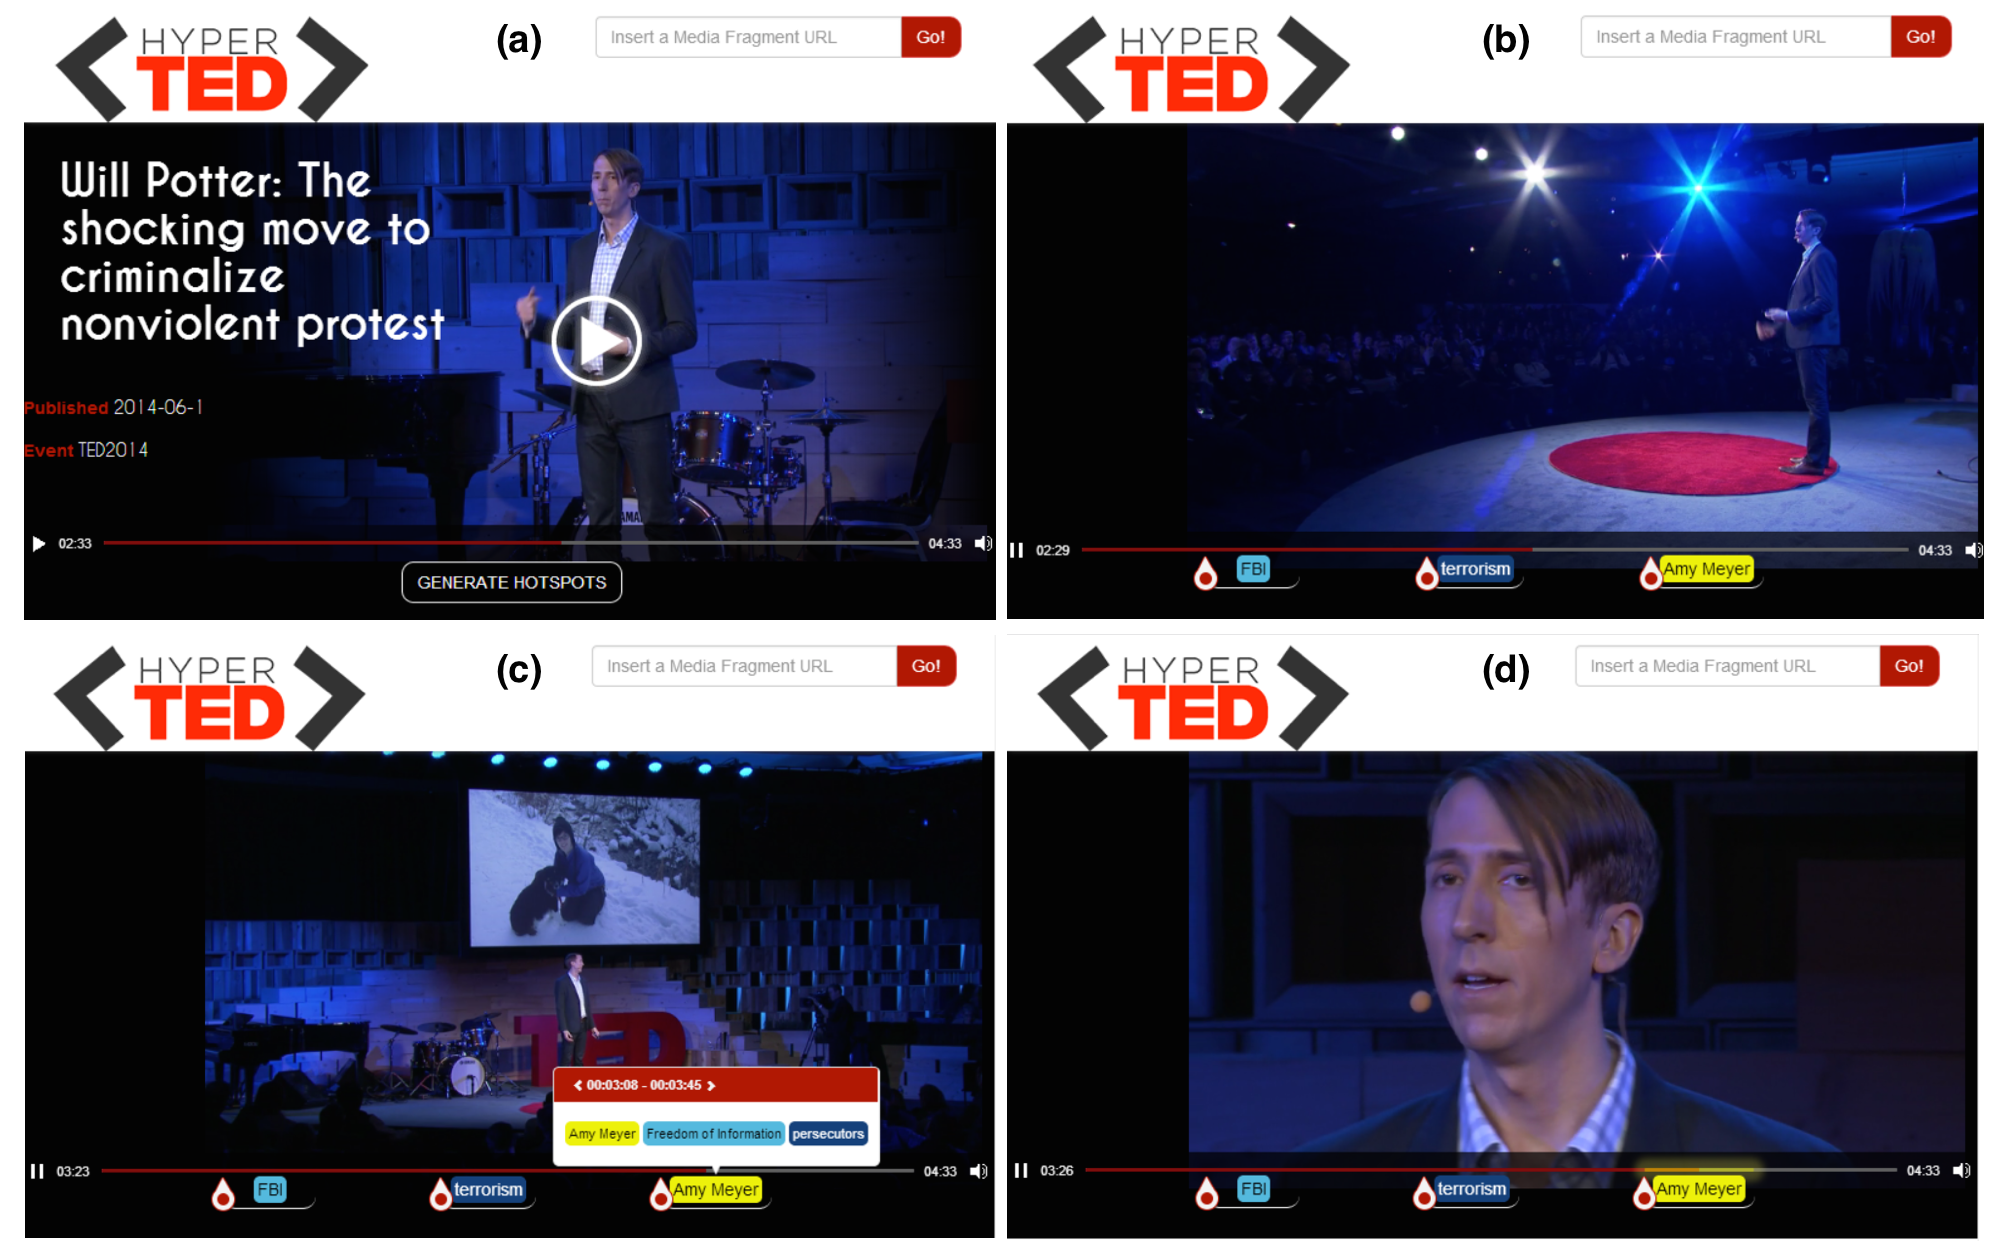
\includegraphics[width=1\textwidth]{figure/Ted_U}
 \caption{Visualizing the Hot Spots of a TED Talk (available at \protect\url{http://linkedtv.eurecom.fr/mediafragmentplayer/video/bbd70fff-e828-4db5-80d0-1a4c9aea430e})}
 \label{fig:demoScreenShots}
\end{figure}

%%%%%%%%%%%%%%%%%%%%%%%
%%%  4. Discussion  %%%
%%%%%%%%%%%%%%%%%%%%%%%

\section{Discussion}
\label{sec:discussion}
We have presented a demo for automatically discovering Hot Spots in online and educational videos. We leverage on visual analysis and background knowledge available in the web of data for detecting what fragments illustrate the best the main topics discussed in the video. Those Hot Spots allow the viewer to quickly decide if a video is worth watching and will provide incentive for consuming videos at the fragment level. In addition, Hot Spots can be explored in a dedicated media fragment player which also display the attached semantic annotations.

We plan to carry out an exhaustive evaluation of our approach involving real users feedback, in order to optimize the results of our Hot Spot detection algorithm and to improve the usability and efficiency of the developed interface. We also plan to further exploit the segmentation results and their corresponding annotations for establishing links between fragments belonging to different videos in order to generate true hyperlinks within a closed collection such as TED talks, and even make results available following Linked Data principles.

%%%%%%%%%%%%%%%%%%%%%%%%%
%%%  Acknowledgments  %%%
%%%%%%%%%%%%%%%%%%%%%%%%%

%\section*{Acknowledgments}
%This work was partially supported by the European Union's 7th Framework Programme via the project LinkedTV (GA 287911).

%%%%%%%%%%%%%%%%%%%%%%
%%%  Bibliography  %%%
%%%%%%%%%%%%%%%%%%%%%%
\bibliographystyle{abbrv}
\bibliography{VideoHotSpots-reduced}

\end{document}
